\documentclass[../revisedmain.tex]{subfiles}
\begin{document}
The shell method is the opposite way to calculate revolved solids of the disc method. If one is given a cross section like this:
\begin{center}
	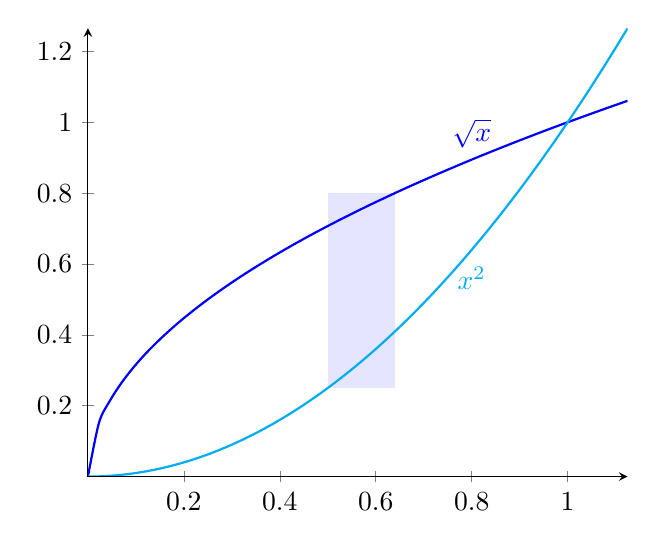
\begin{tikzpicture}
		\begin{axis}[domain=0:1.125,axis lines=middle,axis on top]
		\fill[blue!10] (axis cs:0.5,0.25) rectangle (axis cs:0.64,.8);
		\addplot[smooth,thick,samples=50,blue]{x^0.5};
		\node [anchor=south,color=blue] at (axis cs:.8,.9){$\sqrt{x}$};
		\addplot[smooth,thick,samples=50,cyan]{x^2};
		\node [anchor=south,color=cyan] at (axis cs:.8,.5){$x^2$};
		\end{axis}
	\end{tikzpicture}
\end{center}
An area bounded by two functions revolved around the y-axis, it can be easier to calculate shells instead of discs. We can say that we have approximations for a thin ``shell'' that is just a circle's circumference multiplied by some width. This is not exactly the formula for a shell-like object but because the width is so small, it's practically 2-dimensional and the approximation is close enough. The error becomes closer to 0 as the width of the shells closes in on 0 (a limit!). We end up with the formula for each shell being: $$2*\pi*r*height*width$$The radius in this case is $x$ because every point will be $x$ units away from the $y$-axis, the height will be the top function minus the bottom ($\sqrt{x}-x^2$). The width is an infinitely small amount of $x$, or $dx$. Therefore the formula is:$$2\pi\int_{0}^{1}x(\sqrt{x}-x^2)dx$$  in this case.
\end{document}